\documentclass{beamer}



%\usepackage{beamerthemesplit}
\usetheme{Boadilla}
%\usetheme{default}
%\useinnertheme{rounded}

%\useoutertheme{shadow}
\usecolortheme{rose}
%\usefonttheme{serif}
\setbeamertemplate{navigation symbols}{}
\usetheme{Madrid}

\usepackage{amssymb,amsmath,amscd,amsfonts,amsthm,dsfont,color,graphicx}
\usepackage{amscd}
%\usepackage[numbers]{natbib}
% \usepackage[french]{babel}
%\usepackage[active]{srcltx}


% \date[]{}

 \newcommand\makebeamertitle{\frame{\maketitle}}%

 \AtBeginDocument{
   \let\origtableofcontents=\tableofcontents
   \def\tableofcontents{\@ifnextchar[{\origtableofcontents}{\gobbletableofcontents}}
   \def\gobbletableofcontents#1{\origtableofcontents}
 }
\numberwithin{equation}{section}
  \theoremstyle{plain}
  \newtheorem*{thm*}{\protect\theoremname}
  \theoremstyle{plain}
  \newtheorem*{cor*}{\protect\corollaryname}
 \theoremstyle{definition}
 \newtheorem*{defn*}{\protect\definitionname}
 \theoremstyle{plain}
\newtheorem*{lem*}{\protect\lemmaname}
  \theoremstyle{plain}
  \newtheorem*{rem*}{\protect\remarkname}
   \theoremstyle{definition}
 \newtheorem*{prop*}{\protect\propositionname}

\usetheme{Madrid}

\makeatother

  \providecommand{\corollaryname}{Corollary}
  \providecommand{\definitionname}{Definitioninition}
  \providecommand{\theoremname}{Theorem}
   \providecommand{\lemmaname}{Lemma}
   \providecommand{\remarkname}{Remark}
   \providecommand{\propositionname}{Proposition}
   
   


\newcommand{\Rl}{\mathbb{R}}
\newcommand{\Cplx}{\mathbb{C}}
\newcommand{\Itgr}{\mathbb{Z}}
\newcommand{\Ntrl}{\mathbb{N}}
\newcommand{\Circ}{\mathbb{T}}
\newcommand{\Sb}{\mathbb{S}}
\newcommand{\Disc}{\mathbb{D}}
\newcommand{\Aff}{\mathbb{A}}

% The Caligraphic alphabet
\newcommand{\Ac}{\mathcal{A}}
\newcommand{\Bc}{\mathcal{B}}
\newcommand{\Cc}{\mathcal{C}}
\newcommand{\Dc}{\mathcal{D}}
\newcommand{\Ec}{\mathcal{E}}
\newcommand{\Fc}{\mathcal{F}}
\newcommand{\Gc}{\mathcal{G}}
\newcommand{\Hc}{\mathcal{H}}
\newcommand{\Ic}{\mathcal{I}}
\newcommand{\Jc}{\mathcal{J}}
\newcommand{\Kc}{\mathcal{K}}
\newcommand{\Lc}{\mathcal{L}}
\newcommand{\Mv}{\mathcal{M}}
\newcommand{\Nv}{\mathcal{N}}
\newcommand{\Oc}{\mathcal{O}}
\newcommand{\Pc}{\mathcal{P}}
\newcommand{\Qc}{\mathcal{Q}}
\newcommand{\Rc}{\mathcal{R}}
\newcommand{\Sc}{\mathcal{S}}
\newcommand{\Tc}{\mathcal{T}}
\newcommand{\Uc}{\mathcal{U}}
\newcommand{\Vc}{\mathcal{V}}
\newcommand{\Wc}{\mathcal{W}}
\newcommand{\Xc}{\mathcal{X}}
\newcommand{\Yc}{\mathcal{Y}}
\newcommand{\Zc}{\mathcal{Z}}


\newcommand{\Sp}{\mathrm{Sp}}
\newcommand{\tr}{\mathrm{tr}}
\newcommand{\Op}{\mathrm{Op}}
\newcommand{\sym}{\mathrm{sym}}
\newcommand{\Vol}{\mathrm{Vol}}
\newcommand{\Tr}{\mathrm{Tr}}
\newcommand{\dist}{\mathrm{dist}}
\newcommand{\sgn}{\operatorname{sgn}}
\newcommand{\diag}{\mathrm{diag}}
\newcommand{\id}{\mathrm{id}}
\newcommand{\Poly}{\mathrm{Poly}}

\newcommand{\spec}{\mathrm{Spec}}
\newcommand{\abs}{\mathrm{abs}}

\newcommand{\CV}{\mathrm{CV}}
\newcommand{\PCV}{\mathrm{PCV}}


% Used for highlighting. To remove all highlighting just make the command blank
\newcommand{\hl}{\color{red}}



\newcommand{\dom}{\mathrm{dom}}
\newcommand{\supp}{\mathrm{supp}}
\newcommand{\BS}{\mathfrak{BS}}
\newcommand{\loc}{\mathrm{loc}}
\newcommand{\re}{\mathrm{re}}
\newcommand{\im}{\mathrm{im}}

% DOI transformer
\newcommand{\Ti}{\mathcal{T}}


\def\Xint#1{\mathchoice
{\XXint\displaystyle\textstyle{#1}}%
{\XXint\textstyle\scriptstyle{#1}}%
{\XXint\scriptstyle\scriptscriptstyle{#1}}%
{\XXint\scriptscriptstyle\scriptscriptstyle{#1}}%
\!\int}
\def\XXint#1#2#3{{\setbox0=\hbox{$#1{#2#3}{\int}$ }
\vcenter{\hbox{$#2#3$ }}\kern-.6\wd0}}
\def\qint{\Xint-}

\def\qd{\,{\mathchar'26\mkern-12mu d}}


   
   
   
\begin{document}

\title[$L_p$ estimates in the AMY calculus]{$L_p$ boundedness of operators in the Androulidakis-Mohsen-Yuncken calculus}


\author[E. McDonald]{Ed McDonald}


\institute[]{Penn State University}

\makebeamertitle

\begin{frame}{Introduction}
  This talk is mostly based on my preprint
  \begin{center}
    $L_p$ estimates in the Androulidakis-Mohsen-Yuncken calculus, \href{https://arxiv.org/abs/2410.13701}{arXiv:2410.13701}.
  \end{center}
  In turn, this work was based on the paper by Androulidakis, Mohsen and Yuncken that can be found at \href{https://arxiv.org/abs/2201.12060v2}{arXiv:2201.12060}.
\end{frame}

\section{Asteroids}\label{asteroids_section}

\begin{frame}
  \Huge{Part \ref{asteroids_section}: Asteroids}
\end{frame}

\begin{frame}{Rules of Asteroids}
  In the classic game of asteroids, a player controls a spaceship moving on a two dimensional toroidal space, $\Rl/\Itgr\times \Rl/\Itgr.$ There are two controls available:
  \begin{enumerate}
    \item{} The spaceship can be rotated,
    \item{} The spaceship can be moved forward.
  \end{enumerate}
\end{frame}

\begin{frame}{Configuration space of Asteroids}
  The configuration space of the game is the three-dimensional torus $\Circ^3 = (\Rl/\Itgr)^3,$ with coordinates $(x,y,\theta),$ where $(x,y)$ is the position of the spaceship and $\theta$ is its angle.

  The controls of the game allow us to move along the vector fields
  \[
    X = \cos(\theta)\partial_x+\sin(\theta)\partial_y,\quad Y = \partial_\theta.
  \]
  \pause
  The player moves the spaceship along a path which is parallel to the span of $X$ and $Y.$ That is, the path of the spaceship in configuration space is $\{\gamma(t)\}_{t\geq 0},$ where
  \[
    \dot{\gamma}(t) \in \mathrm{span}\{X_{\gamma(t)},Y_{\gamma(t)}\},\quad t\geq 0.
  \]
  \pause
  Despite there being only two available directions, we can reach any point $(x,y,\theta)$ from any other point by traveling on a piecewise-smooth path parallel to $X$ and $Y.$
  \pause
  Physically, this is called a \emph{non-holonomic constraint}.
\end{frame}

\begin{frame}{Asteroids}
  In general, if we can travel parallel to $X$ and $Y$ then we can approximate paths along $[X,Y],$ by the Lie-Kato-Trotter product formula
  \[
    \exp(t[X,Y]) = \lim_{n\to\infty} (\exp(\frac{t}{n}X)\exp(\frac{t}{n}Y)\exp(-\frac{t}{n}(X+Y))\exp(-\frac{t}{n}Y))^n.
  \]
  But moving along $[X,Y]$ is harder than moving along $X$ and $Y.$

  In the asteroids example,
  \[
    [X,Y] = \sin(\theta)\partial_x-\cos(\theta)\partial_y
  \]
  so $\{X,Y,[X,Y]\}$ form a basis for the tangent space to $\Circ^3$ at every point.
\end{frame}

\begin{frame}{Random walks}
  A random walk making independent increments in the $X$ and $Y$ directions looks a bit like this:
  \begin{center}
  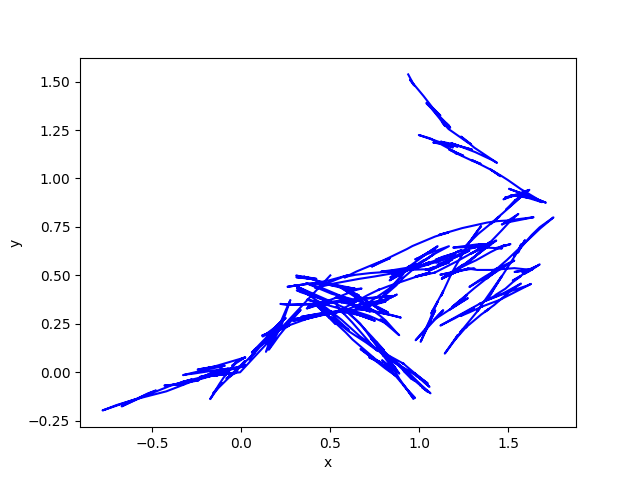
\includegraphics[width=90mm]{xy_coords_single_paths.png}
  \end{center}
%   (this is displayed in ``unwrapped" coordinates, i.e. we do not take the quotient modulo $\Itgr^2.$).
\end{frame}

\begin{frame}{Random walks}
  Ten realisations of the same random walk look like this:
  \begin{center}
    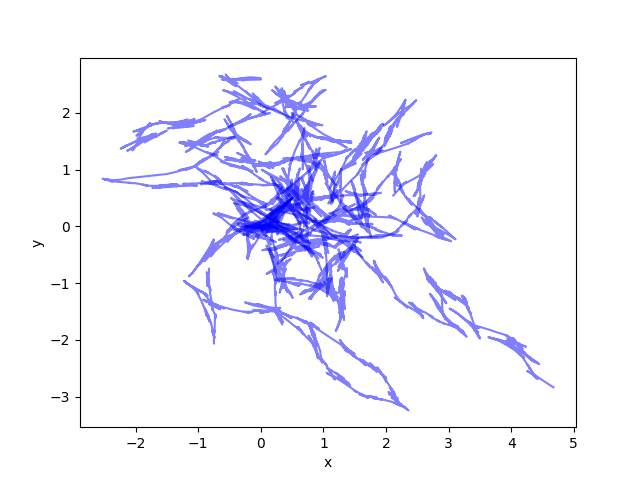
\includegraphics[width=90mm]{xy_coords_multiple_paths.png}
  \end{center}
\end{frame}

\begin{frame}{Random walks}
  The path through configuration space is in three dimensions, and looks like this:
  \begin{center}
  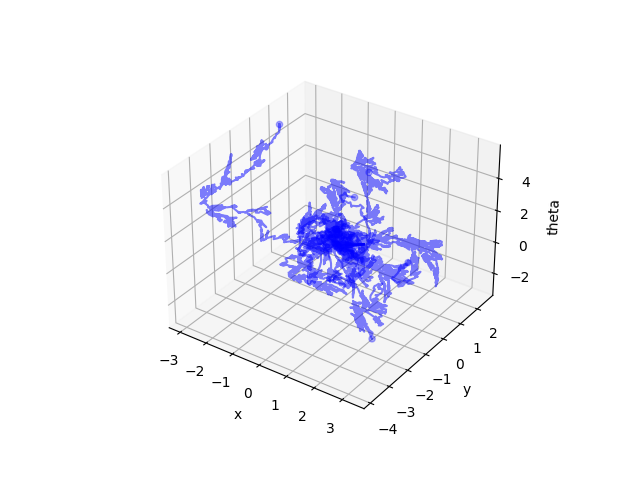
\includegraphics[width=90mm]{xyt_coords_multiple_paths.png}
  \end{center}
%   (again, the picture is of $\Rl^3$ rather than $\Circ^3$ for clarity).
\end{frame}

\begin{frame}{Asteroids}
  Thinking about $X$ and $Y$ as derivations (not just as directions), we should think of $X,Y$ as being order $1$ and $[X,Y]$ as being order $2.$

  The operator
  \[
    \Theta = X^2+Y^2 = \partial_\theta^2+(\cos(\theta)\partial_x+\sin(\theta)\partial_y)^2
  \]
  is homogeneous of order $2.$
  \pause
  \begin{center}
      $\Theta$ is not elliptic, but $(1-\Theta)^{-1}$ does improve regularity somewhat. Why, and by how much?
  \end{center}
  \pause
  In stochastic analysis, $\Theta$ is the generator of the random walks above.
\end{frame}

\begin{frame}{Asteroids}
 Let $\|u\|_{W^s_2(\Circ^3)}$ denote the standard Hilbert-Sobolev norm of order $s\in \Rl$ of $u\in C^\infty(\Circ^3).$ That is,
 \[
      \|u\|_{W^s_2(\Circ^3)} := \|(1-\partial_x^2-\partial_y^2-\partial_\theta^2)^{\frac{s}{2}}u\|_{L_2(\Circ^3)}.
 \]
 A highly non-trivial calculation gives us the \emph{sub-elliptic estimates}:
  \[
      \|u\|_{W^{s+\frac12}_2(\Circ^3)}\lesssim_s \|\Theta u\|_{W^s_2(\Circ^3)}+\|u\|_{W^s_2(\Circ^3)}.
  \]
  This implies hypoellipticity (i.e., $\Theta u\in C^\infty \Rightarrow u \in C^\infty$.)
\end{frame}

\begin{frame}{More examples}
  A similar example can be seen on the Lie group $\mathrm{SO}(3).$ The Lie algebra $\mathfrak{so}(3)$
  is spanned by three elements, $\{A,B,C\},$ and $[A,B]=C, [C,A] = B,$ etc.
  \pause
  The operator
  \[
      \Delta = A^2+B^2+C^2
  \]
  is the \emph{quadratic Casimir element}. It is elliptic.
  \pause
  The operator
  \[
    \Theta = A^2+B^2
  \]
  is not elliptic, but it is hypoelliptic.
\end{frame}
% 
% \begin{frame}
%     \huge{Section 1: Carnot-Carath\'eodory geometry and maximal hypoellipticity}
% \end{frame}
% 
% \begin{frame}{Geometry defined by vector fields}
%   Let $U\subset \Rl^d$ be open, and let $X_1,\ldots,X_N$ be smooth vector fields on $U.$
%   Assume that $X_1,\ldots,X_N$ span the tangent space at every point, and equip each vector field with a weight $\{w_1,\ldots,w_N\}.$ 
% \end{frame}



\section{Pseudodifferential calculus}\label{psido_section}

\begin{frame}
    \huge{Section \ref{psido_section}: Pseudodifferential calculus}
\end{frame}

\begin{frame}{What is a pseudodifferential calculus?}
  One of the best ways of studying differential operators is to build a pseudodifferential calculus.
  \pause
  Let $M$ be a closed manifold, and let $\mathrm{DO}^k(M)$ be the set of differential operators on $M$
  of order $k\geq 0.$ That is, locally $P \in \mathrm{DO}^k(M)$ looks like
  \[
    P = \sum_{|\alpha|\leq k} a_{\alpha}(x)\partial^{\alpha}.
  \]
  Let $\mathrm{DO}(M) = \bigcup_{k\geq 0} \mathrm{DO}^k(M).$
  \pause
  We could also count ``orders" in a non-traditional way as in the Asteroids example, where $X$ and $Y$ have order $1$ and $[X,Y]$ has order $2.$
\end{frame}

\begin{frame}{What is a pseudodifferential calculus?}
  $\mathrm{DO}(M)$ is a filtered algebra. That is, $\mathrm{DO}^{k}(M)\subset \mathrm{DO}^{k+1}(M)$ and
  \[
    \mathrm{DO}^k(M)\cdot \mathrm{DO}^\ell(M) \subseteq \mathrm{DO}^{k+\ell}(M).
  \]
  What we would like to do is embed $\mathrm{DO}(X)$ into a larger filtered algebra $\Psi(M)=\bigcup_{k\in \Itgr} \Psi^k(M),$ with
  \[
    \mathrm{DO}^k(M) \subseteq \Psi^k(M).
  \]
\end{frame}

\begin{frame}
  Desirable properties include:
  \begin{itemize}
    \item{} $\Psi^k(M)$ should be closed under the adjoint
    \item{} $\Psi^0(M)$ should act as bounded operators on $L_2(M).$
    \item{} $\Psi^{-\infty}(M)$ consists of smoothing operators.
    \item{} Negative order operators should be compact.
  \end{itemize}\pause
  The final three conditions can be included in:
  \begin{itemize}
    \item{} $\Psi^k(M)$ acts boundedly from $W^{s+k}_2(M)$ to $W^{s}_2(M)$ for all $s\in \Rl.$
  \end{itemize}
\end{frame}

\begin{frame}{What is a pseudodifferential calculus?}
  The most important thing that we want is 
  \begin{itemize}
    \item{} Elliptic operators $D\in \mathrm{DO}^k(M)$ should have a parametrix $Q \in \Psi^{-k}(M).$
  \end{itemize}
  A parametrix is an inverse modulo smoothing, i.e.
  \[
    DQ-1,QD-1 \in \Psi^{-\infty}(M).
  \]
  \pause
  In the standard calculus, $P=\sum_{|\alpha|\leq k} a_{\alpha}(x)\partial^{\alpha}$ is elliptic if its principal symbol is invertible, i.e.
  \[
    \xi\neq 0\Rightarrow \sum_{|\alpha|=k} a_{\alpha}\xi^{\alpha} \neq 0.
  \]
\end{frame}

\begin{frame}{Why a pseudodifferential calculus?}
  There are a lot of things to be done with a pseudodifferential calculus. One of the most important is in deriving \emph{elliptic estimates}.
  \begin{lemma}
    Suppose that $\Psi(M) = \bigcup_{k\in \Itgr} \Psi^k(M)$ is a pseudodifferential calculus satisfying all of the desirable conditions above. If $D\in \mathrm{DO}^k(M)$ is elliptic, then for every $s \in \Rl$ there exists a constant $C_{s,D}$ such that
    \[
      \|u\|_{W^{s+k}_2(M)} \leq C_{s,D}(\|Du\|_{W^s_2(M)} + \|u\|_{W^{s}_2(M)}).
    \]
  \end{lemma}
  \pause
  In PDE terms, these estimates imply the \emph{a priori regularity} of solutions to the equation $Du=f.$ That is, if $u\in \Dc'(M),$ $f \in W^s_2(M)$ and $Du=f,$ then $u\in W^{s+k}_2(M).$
\end{frame}
\begin{frame}{Why a pseudodifferential calculus?}
  \begin{proof}
    Let $Q$ be a parametrix for $D.$ For $u\in C^\infty(M),$ write
    \[
        u = QDu+(1-QD)u.
    \]  
    \pause
    Since $Q$ and $1-QD$ are bounded from $W^{s+k}_2(M)$ to $W^{s}_2(M),$ it follows that
    \begin{align*}
        \|u\|_{W^{s+k}_2(M)} &\leq \|Q\|_{W^{s+k}_2(M)\to W^s_2(M)}\|Du\|_{W^s_2(M)}\\
        &\quad +\|1-QD\|_{W^{s+k}_2(M)\to W^s_2(M)}\|u\|_{W^s_2(M)}.
    \end{align*}
  \end{proof}
\end{frame}

\begin{frame}{Elliptic estimates in $L_p$-spaces}
    $L_2$ Sobolev spaces are the easiest to deal with since they are Hilbert spaces, but there are reasons to want $L_p$ elliptic estimates, too. For an elliptic operator $D\in \mathrm{DO}^k(M),$ $L_p$ elliptic estimates take the form
    \[
        \|u\|_{W^{s+k}_p(M)} \leq C_{s,D,p}(\|Du\|_{W^{s}_p(M)}+\|u\|_{W^{s}_p(M)}).
    \]
    \pause
    From the above argument, the key to proving these estimates is to show that operators in $\Psi^k(M)$ act boundedly from $W^{s+k}_p(M)$
    to $W^{s}_p(M)$ for every $s\in \Rl.$
\end{frame}

\begin{frame}{Why elliptic estimates in $L_p$-spaces?}
    We need Sobolev spaces $W^s_p(M)$ for $p\neq 2$ for nonlinear PDE. 
    \pause
    Consider $P\in \mathrm{DO}^2(M),$ where $P = -\sum_{j=1}^d X_j^2,$ and the $X_j$ are vector fields on $M.$ Suppose that $P$ is elliptic.
    \pause
    Let $f \in C^\infty(M).$ Using variational methods, it is easy to show that the PDE
    \[
        Pu+u^3 = f
    \]
    has a weak solution $u$ belonging to $L_4(M).$ In order to show that $u$ is a classical solution, we need to show that it has two orders of differentiability.
    \pause
    If we know elliptic estimates in $p=\frac{4}{3},$ then
    \begin{align*}
        \|u\|_{W^2_{\frac{4}{3}}(M)} &\lesssim \|Pu\|_{L_{\frac{4}{3}}(M)}+\|u\|_{L_{\frac{4}{3}}(M)}\\
                                     &\lesssim \|f\|_{L_{\frac{4}{3}}}+\|u\|_{L_4(M)}.
    \end{align*}
\end{frame}

\begin{frame}{How to build a pseudodifferential calculus}
    Specialise to $M = \Rl^d.$ \pause ($^*$ not compact, but close enough.)
    \pause
    It is easy enough to build parametrices for \emph{constant coefficient} differential operators. These can be realised as convolution operators
    \[
        \Op(k)u(x) := \int_{\Rl^d} k(z)u(x+z)\,dz,\quad u\in C^\infty_c(\Rl^d).
    \]
    Here, $k$ is a distribution on $\Rl^d$ and the integral should be interpreted as distributional pairing.
\end{frame}

\begin{frame}{How to build a pseudodifferential calculus}
    To build parametrices for non-translation-invariant operators, we need to consider operators of the form
    \[
        \Op(K)u(x) = \int_{\Rl^d} K(x,z)u(x+z)\, dz,\quad u\in C^\infty_c(\Rl^d)
    \]
    where $K$ is smooth in the $x$-variable and potentially singular in the $z$ variable.
\end{frame}

\begin{frame}{How to build a pseudodifferential calculus}
    In general, for operators on a manifold $M$ we need to consider
    \[
        \Op(K)u(x) = \int_{TM_x} K(x,z)u(\exp_xz)\,dz,\quad u\in C^\infty_c(M)
    \]
    where $K$ is a distribution on the tangent bundle $TM,$ and $\exp_x$ is an exponential mapping.
\end{frame}

\begin{frame}{How to build a pseudodifferential calculus}
    This leads to the question: what are the right conditions on a kernel $K$ which ensure that all the operators of the form $\Op(K)$ form a good pseudodifferential calculus? \pause
    Following a suggestion from Androulidakis and Skandalis, it turns out that a good idea is to introduce another parameter.
    \begin{theorem}[Van Erp-Yuncken (2019)]
        Consider the class of distributions $(x,z,\hbar) \mapsto K(x,z,\hbar)$ which are smooth in $(x,\hbar)$ and compactly supported in $z.$ If for all $\lambda>0$ the difference
        \[
            \lambda^{-k-d}K(x,\lambda^{-1}z,\lambda \hbar)-K(x,z,\hbar)
        \]
        is smooth in $(x,z,\hbar),$ then $K(x,\cdot,1)$ is the kernel of a classical pseudodifferential operator of order $k.$
        
        Conversely, every classical pseudodifferential operator arises in this way.
    \end{theorem}
\end{frame}

\begin{frame}{Filtered pseudodifferential calculus}
    One of the advantages of the van Erp-Yuncken point of view is that it generalises neatly to non-traditional weightings. 
    \pause
    
    Let $0=H^0<H^1 < \cdots < H^N = TM$ be a filtration of the tangent bundle of a manifold $M.$ Let $\mathrm{DO}_H(M) = \bigcup_{k\geq 0} \mathrm{DO}_H^k(M)$ be the algebra of differential operators with orders counted so that vector fields in $H^j$ have order $j,$ for all $1\leq j\leq N.$ There is a natural notion of ``elliptic" for $\mathrm{DO}_H(M)$ (the Rockland condition). There is also a natural scale of Sobolev spaces adapted to the filtration.
        \pause
    \begin{theorem}
        There exists a pseudodifferential calculus $\Psi_H(M) = \bigcup_{k\in \Itgr} \Psi^k_H(M)$ extending $\mathrm{DO}_H(M),$ 
        with all of the desirable properties described above.
    \end{theorem}
    \pause
    (Pseudodifferential calculi for this and similar situations have been described by Folland, Rothschild, Stein, Melin, Goodman, Beals, Greiner, Stanton, Taylor, Ponge, Street, and others. Van Erp and Yuncken's contribution is in simplifying the definition.)
\end{frame}

\begin{frame}{The asteroids example}
  In the Asteroids example, we have $M=\Circ^3,$ and the sections of $H^1$ and $H^2$ are given by
  \[
    \Gamma H^1 = \mathrm{span}\{X,Y\},\quad \Gamma H^2 = \mathrm{span}\{\Gamma H^1, [X,Y]\}.
  \]
\end{frame}

\section{Operators defined by submersions}\label{submersion_section}

\begin{frame}
    \huge{Section \ref{submersion_section}: Operators defined by submersions}
\end{frame}

\begin{frame}{Limitations of the exponential map}
    Recall that pseudodifferential operators on a manifold $M$ were defined by some choice of exponential map $\exp_x$ by 
    \[
        \Op(K)u(x) = \int_{TM_x} K(x,z)u(\exp_x(z))\,dz.
    \]
    There are lots of circumstances where we need to integrate over a space of dimension larger than $TM_x,$ so that operators are locally defined by integrals of the form
    \[
        \Op(K)u(x) = \int_V K(x,z)u(\Lambda_x(z))\,dz
    \]
    where $V$ is a linear space and $\mathrm{dim}(V)\geq \mathrm{dim}(M),$ $K$ is a distribution on $M\times V,$ and $\Lambda_x:V\to M$ is a submersion, smoothly depending on $x \in X.$   
\end{frame}

\begin{frame}{Example: the Grushin operator}
    The operator on $\Rl^2$ with coordinates $(x,y)$ given by
    \[
        G = \partial_x^2+x^2\partial_y^2
    \]
    is called the \emph{Grushin operator}. We can write it as a sum of squares of vector fields,
    \[
        G = X_1^2+X_2^2,\quad X_1 := \partial_x,\; X_2 := x\partial_y.
    \]
    $X_1$ and $X_2$ do not span the tangent space at points where $x=0.$ Instead we need to include a third vector field
    \[
        X_3 := [X_1,X_2] = \partial_y.
    \]
\end{frame}

\begin{frame}{Example: the Grushin operator}
    The natural differential calculus associated to the Grushin operator is built in the following way: let $K$ be a distribution on $\Rl^2\times \Rl^3,$ and let
    \[
        \Op(K)u(x) = \int_{\Rl^3} K(x,z)u(\exp(z_1X_1+z_2X_2+z_3X_3)x)\,dz,\quad u\in C^\infty_c(\Rl^2).
    \]
    where $\exp$ is the exponential of vector fields.
\end{frame}

\begin{frame}{The AMY calculus for the Grushin operator}
\begin{theorem}
    Let $(x,z,\hbar)\mapsto K(x,z,\hbar)$ denote a distribution on $\Rl^2\times\Rl^3\times \Rl$ which is smooth in $(x,\hbar)$ and compactly supported in $z.$ Assume that for every $\lambda>0$ the difference
    \[
        \lambda^{-k-4}K(x,\lambda^{-1}z_1,\lambda^{-1}z_2,\lambda^{-2}z_3,\lambda\hbar)-K(x,z,\hbar)
    \]
    is a smooth function of $(x,z,\hbar).$ Let $\Psi^k$ denote the operators of the form 
    \[
        \Op(K)u(x) = \int_{\Rl^3} K(x,z)u(\exp(z_1X_1+z_2X_2+z_3X_3)x)\,dz,\quad u\in C^\infty_c(\Rl^2).
    \]
    Then $\Psi = \bigcup_{k\in \Itgr} \Psi^k$ has all$^*$ of the desirable properties of a pseudodifferential calculus.
\end{theorem}
\pause
($^*$ The definition of ellipticity is complicated in this example, and they did not prove that elliptic operators have parametrices in the calculus.)
\end{frame}

\begin{frame}{The general case}
    In general, let $U\subset \Rl^d$ be an open subset. Let $X_1,\ldots,X_N$ be smooth vector fields on $U$ which span the tangent space at every point. Let $\{w_1,\ldots,w_N\}$ be positive integers. Say that $X_j$ has weight $w_j.$ 
    \pause
    Similar to the Grushin example, we can build an algebra of operators of the form
    \[
        \Op(K)u(x) = \int_{\Rl^N} K(x,z)u(\exp(z_1X_1+\cdots+z_NX_N)x)\,dz.
    \]
    An ``approximate homogeneity" condition, taking into account the weights, gives a nice pseudodifferential calculus $\Psi(U).$
    \pause
    
    
    A similar pseudodifferential calculus for the same situation was described by Street. It is unclear (to me) what the relationship is between the two constructions.
\end{frame}

\begin{frame}{$L_p$ estimates}
    Finally, I can promote my own work:
    \begin{theorem}[M. (2024)]
        Order zero operators in the AMY calculus are bounded on $L_p$ spaces, for $1<p<\infty.$
    \end{theorem}
    This implies (although not obviously) $L_p$ elliptic estimates for certain differential operators like the Grushin operator, and also some nonlinear PDE.
\end{frame}

\begin{frame}{$L_p$-estimates}
  \begin{corollary}
    Order $k$ operators in the AMY calculus are bounded from $W^{s+k}_p(U)$ to $W^s_p(U)$ for all $s \in \Rl,$
    and elliptic$^*$ operators obey $L_p$ elliptic estimates.
  \end{corollary}
  \pause
  ($^*$ ellipticity really means ``maximal hypoellipticity")
\end{frame}

\begin{frame}
\structure{\begin{center}
{\Huge{}Thank you for listening!}
\par\end{center}}\end{frame}



\end{document}
